\documentclass[12pt,a4paper]{article}

\usepackage{polski}
\usepackage[utf8]{inputenc}
\usepackage{indentfirst}

\usepackage{lscape}
\usepackage{longtable}
\usepackage{blindtext}
\usepackage{graphicx}
\usepackage{caption}
\usepackage{xparse,nameref}
%\usepackage{mathptmx}
%\usepackage[scaled=.90]{helvet}
%\usepackage{xcolor}
\usepackage{titlesec}
\usepackage{listings}
\usepackage{tocloft}
\usepackage{geometry}
\usepackage[nottoc,numbib]{tocbibind}

\DeclareGraphicsExtensions{.pdf,.png,.jpg}

\makeatother

\geometry{a4paper, total={210mm,297mm}, left=25mm, right=25mm, top=25mm, bottom=25mm} % Margins

\lstset{
    basicstyle=\footnotesize\ttfamily,
    breakatwhitespace=false,
    breaklines=true,
    escapeinside={\%*}{*)},
    extendedchars=true,
    frame=l,
    xleftmargin=\parindent,
    keepspaces=true,
    numbers=left,
    numbersep=10pt,
    showspaces=false,
    showstringspaces=false,
    showtabs=false,
    stepnumber=1,
    tabsize=4
}

%\newcommand*\emptypage{\newpage\null\thispagestyle{empty}\newpage}

\NewDocumentCommand{\chapref}{s m}{rozdziale~\ref{#2}\IfBooleanF{#1}{ - \nameref{#2}}, na stronie \pageref{#2}}

\renewcommand*{\thesection}{\arabic{section}}
\renewcommand*{\thesubsection}{\arabic{section}.\arabic{subsection}}
\renewcommand*{\thesubsubsection}{\arabic{section}.\arabic{subsection}.\arabic{subsubsection}}
\renewcommand*\thetable{\arabic{table}}
\renewcommand*\theequation{\arabic{equation}}
\renewcommand*\thefigure{\arabic{figure}}

% \titleformat{\chapter}[display]
%     {\normalfont\sffamily\Large}
%     {\chaptertitlename\ \thechapter}{14pt}{\bfseries\LARGE}
\titleformat{\section}
    {\normalfont\large\bfseries}
    {\thesection}{1em}{}

\title{Demistyfikacja steganografii}
\author{Marek Dalewski}
\date{14 kwietnia 2017}

\begin{document}
\maketitle

\tableofcontents

\renewcommand*{\thelstlisting}{\arabic{lstlisting}}

%\Blinddocument % for style tests

\section{Wstęp}
    Niniejszy tekst powstał jako wprowadzenie dla osób nie nieposiadających technicznego wykształcenia, chcących zapoznać się z~tematyką ukrywania cyfrowych informacji - steganografii cyfrowej.

\section{Czym jest steganografia?}
    To nauka o~ukrywaniu faktu prowadzenia komunikacji.

    To tyle - powyższy akapit w~pełni oddaje cały zakres steganografii, jest sformułowany prostym i~przystępnym językiem, a~jednak nie pozostawia czytelnika usatysfakcjonowanego. Dzieje się tak dlatego, że opis jest zbyt abstrakcyjny, a~dokładniej operuje nieznaną czytelnikowi abstrakcją. Bo jak komunikacja jest ukrywana? Jaka komunikacja? I~co to w~ogóle znaczy ukrywać komunikację?

    Jak więc wytłumaczyć to pojęcie? Może studium uproszczonego przypadku? Tak, by dać praktyczny przykład bez stawiania wymagań specyficznej wiedzy technicznej. Wydaje się to dobry pomysł, jednak na ogół wprowadzanie owych uproszczeń usuwa z~przykładu to, co dla odbiorcy najistotniejsze. Odbiorca, posiadający wymaganą wiedzę techniczną, czy też nie, chce zapoznać się z~tematem z~jakiegoś powodu i~na ogół przyczyna jest znacznie mniej błaha niż zaspokojenie ciekawości. Problem jednak w~tym, jak wytłumaczyć temat, czy chociaż do niego wprowadzić czytelnika w~obliczu postawionego wcześniej założenia nie posiadania wiedzy technicznej. Cóż, pozostaje tylko spróbować wytłumaczyć możliwie przystępnym językiem pełny, a~nie uproszczony przykład.

    Zacznijmy jednak od przedstawionej wcześniej definicji. Według niej mamy tu do czynienia z~komunikacją i~chodzi o~jakąkolwiek komunikację - wymianę tekstów albo na przykład obrazów między dwiema osobami. W~dalszym przykładzie wykorzystamy właśnie obrazy. Osoby mogą używać dowolnego medium komunikacyjnego, na przykład poczty e-mail. Nadal jednak nie wytłumaczyliśmy pojęcia ukrywania. Co to ma oznaczać? Uciekniemy się do prostej sztuczki - by ukryć jedną komunikację użyjemy innej. Oryginalny komunikat ukryjemy w~szumie komunikacyjnym, który sami wygenerujemy. Jak będzie to dokładnie wyglądać w~przykładzie? Ukryjemy nasz oryginalny komunikat (oryginalną wiadomość) - obraz w~innym obrazie.

    Zanim jednak do tego przejdziemy, musimy wytłumaczyć kilka niezbędnych pojęć na temat budowy obrazów cyfrowych.

\section{Notka o~budowie obrazów}
    By przejść do omawiania samego algorytmu ukrywania obrazu w~obrazie, musimy ustalić wspólny poziom wiedzy co do budowy samych obrazów. To, co trzeba wiedzieć, to że obrazy składają się z~pikseli. Z~kolei piksel to taki jednokolorowy kwadracik\footnote{Na potrzeby niniejszej dyskusji całkowicie pominiemy dokładną definicję piksela i~fakt, że piksel niekoniecznie musi być kwadratowy. Ponadto warto zaznaczyć, że - zależnie od formatu graficznego - piksele są przetwarzane przed zapisaniem do pliku (na przykład przez algorytm stratnej albo bezstratnej kompresji).}, a~kolor jednoznacznie charakteryzują trzy liczby\footnote{By nie zakłócać przykładu niepotrzebnymi informacjami, pominiemy tu fakt, że istnieją inne reprezentacje przestrzeni barw, niż użyta tu 24 bitowa reprezentacja RGB.}. Każda z~zakresu od 000 do 255 (każda składa się z~trzech cyfr). Odpowiadają one natężeniu odpowiednio barwy czerwonej, zielonej i~niebieskiej (rysunek \ref{fig:piksel}).

    W~skrócie: piksel, podstawowy atom obrazu, jest kwadracikiem jednego koloru i~można go scharakteryzować przy użyciu trzech liczb z~zakresu od 000 do 255.

% % WB-ONLY START
%     \begin{figure}[!h]
%         \centering
%         \includegraphics[width=0.7\textwidth]{pieces/piksel-cb}
%         \caption{Obraz i~jego piksele} \label{fig:piksel}
%     \end{figure}
% % WB-ONLY END

% COLOR-ONLY START
    \begin{figure}[!h]
        \centering
        \includegraphics[width=0.7\textwidth]{pieces/piksel}
        \caption{Obraz i~jego piksele} \label{fig:piksel}
    \end{figure}

    Warto też zwrócić uwagę na różnicę między kolorami w~miarę zwiększania między nimi odległości\footnote{Termin ``zwiększanie odległości między kolorami'' może budzić wiele wątpliwości. Zauważmy, że możemy interpretować kolor z~palety barw RGB jako punkt w~trójwymiarowej przestrzeni. Gdy mamy dwa kolory, tj. dwa punkty w~przestrzeni, możemy mówić o~odległości między nimi.} - jak niewielkie zachodzą różnice wizualne (rysunek \ref{fig:kolory}).

    \begin{figure}[!h]
        \centering
        \includegraphics[width=0.7\textwidth]{pieces/kolory}
        \caption{Różnice wizualne między kolorami, w~miarę zwiększania odległości między nimi} \label{fig:kolory}
    \end{figure}
% COLOR-ONLY END

\section{Algorytm ukrywający dane}
    Po zapoznaniu się z~budową obrazów cyfrowych, nie pozostaje już nic innego, niż przejść do metody steganograficznej i~rozpocząć ukrywanie danych. Sposób postępowania jest następujący\footnote{Stosowane nazewnictwo obrazów jest następujące: ``obraz z~wiadomością'' to obraz, który \textbf{jest ukrywany}; ``obraz oryginalny'' to obraz, \textbf{w którym ukrywamy}.}:
    \begin{enumerate}
        \item Wybieramy piksel obrazu z~ukrywaną wiadomością i~odpowiadające mu trzy piksele w~oryginalnym obrazie\footnote{Obraz oryginalny musi być co najmniej trzy razy szerszy, by każdy piksel obrazu z~wiadomością znalazł odpowiadające mu trzy piksele obrazu oryginalnego.} (rysunek \ref{fig:wybor-pikseli}).
        \item Zerujemy cyfrę jedności dla każdego kanału koloru, dla każdego piksela z~obrazu oryginalnego (rysunek \ref{fig:zerowanie-pikseli}).
        \item Zgodnie z~rysunkiem \ref{fig:wstawianie-pikseli} wstawiamy cyfry z~piksela obrazu z~wiadomością do pikseli obrazu oryginalnego.
    \end{enumerate}
    Powyższe czynności powtarzamy dla wszystkich pikseli w~obrazie z~wiadomością.

    By wyeksportować ukryte wcześniej dane i~odzyskać oryginalny obraz z~wiadomością, wystarczy odwrócić przedstawione kroki.

% % WB-ONLY START
%     \begin{figure}[!h]
%         \centering
%         \includegraphics[width=0.7\textwidth]{pieces/wybor-pikseli-cb}
%         \caption{Piksel obrazu z~wiadomością wraz z~odpowiadającymi mu pikselami oryginalnego obrazu} \label{fig:wybor-pikseli}
%     \end{figure}

%     \begin{figure}[!h]
%         \centering
%         \includegraphics[width=0.7\textwidth]{pieces/zerowanie-pikseli-cb}
%         \caption{Zerowanie jedności w~pikselach obrazu oryginalnego} \label{fig:zerowanie-pikseli}
%     \end{figure}

%     \begin{figure}[!h]
%         \centering
%         \includegraphics[width=0.7\textwidth]{pieces/wstawianie-pikseli-cb}
%         \caption{Schemat wstawiania cyfr} \label{fig:wstawianie-pikseli}
%     \end{figure}
% % WB-ONLY END

% COLOR-ONLY START
    \begin{figure}[!h]
        \centering
        \includegraphics[width=0.7\textwidth]{pieces/wybor-pikseli}
        \caption{Piksel obrazu z~wiadomością wraz z~odpowiadającymi mu pikselami oryginalnego obrazu} \label{fig:wybor-pikseli}
    \end{figure}

    \begin{figure}[!h]
        \centering
        \includegraphics[width=0.7\textwidth]{pieces/zerowanie-pikseli}
        \caption{Zerowanie jedności w~pikselach obrazu oryginalnego} \label{fig:zerowanie-pikseli}
    \end{figure}

    \begin{figure}[!h]
        \centering
        \includegraphics[width=0.7\textwidth]{pieces/wstawianie-pikseli}
        \caption{Schemat wstawiania cyfr} \label{fig:wstawianie-pikseli}
    \end{figure}
% COLOR-ONLY END

    Powyższa metoda jest bardzo prosta, a~zarazem jest to jeden z~najczęściej spotykanych algorytmów steganograficznych. Jego wadą jest łatwość wykrycia, gdy tylko znamy metodę ukrywania. Istnieją oczywiście dużo bardziej zaawansowane i~bezpieczniejsze metody. Bazują one jednak na zaawansowanych przekształceniach matematycznych, których przytaczanie, na potrzeby krótkiego wprowadzenia do tematu jest bezzasadne.

% COLOR-ONLY START
\section{Demonstracja algorytmu}
    Na rysunku \ref{fig:stegano-rezultat} możemy zobaczyć rezultat działania powyższego algorytmu dla obrazu oryginalnego (rysunek \ref{fig:stegano-zrodlo}) i~obraz z~wiadomością (rysunek \ref{fig:stegano-wiadomosc}). Zwróćmy uwagę, że zmian wprowadzonych działaniem algorytmu nie widać gołym okiem.

    \begin{figure}[!h]
        \centering
        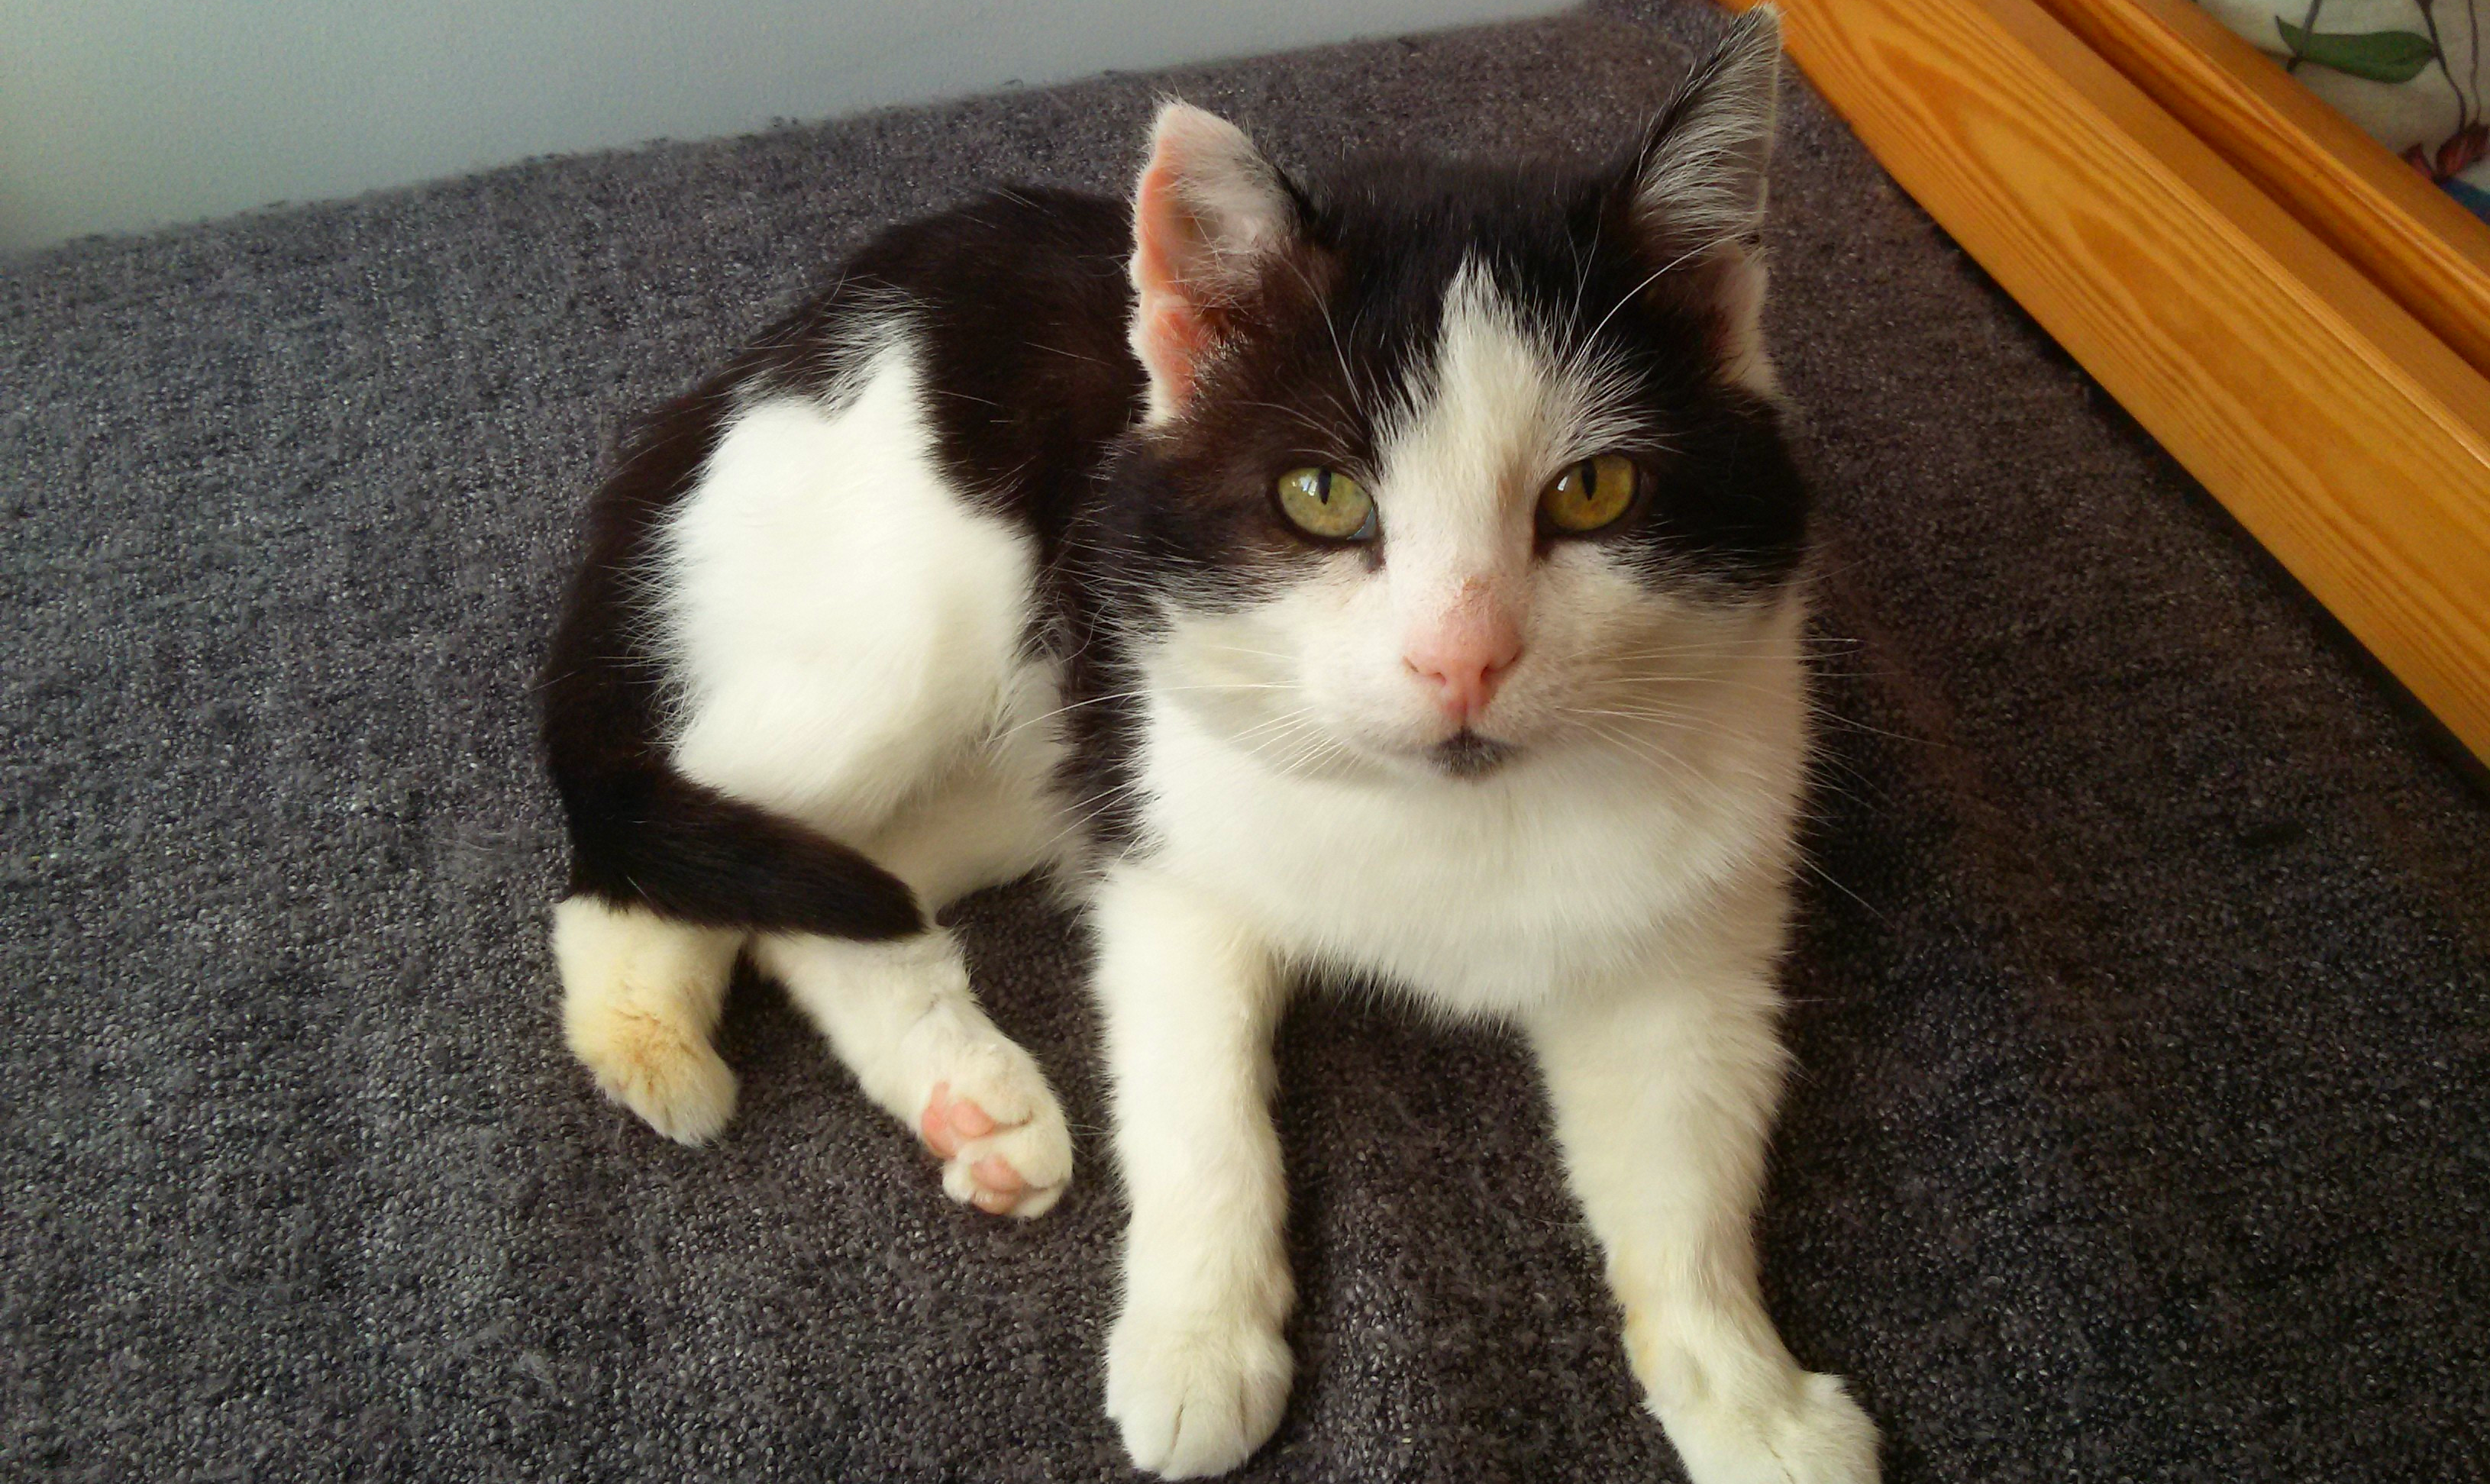
\includegraphics[width=0.4\textwidth]{pieces/kot}
        \caption{Obraz oryginalny} \label{fig:stegano-zrodlo}
    \end{figure}

    \begin{figure}[!h]
        \centering
        \includegraphics[width=0.2\textwidth]{pieces/wiadomosc}
        \caption{Obraz z~wiadomością do ukrycia} \label{fig:stegano-wiadomosc}
    \end{figure}

    \begin{figure}[!h]
        \centering
        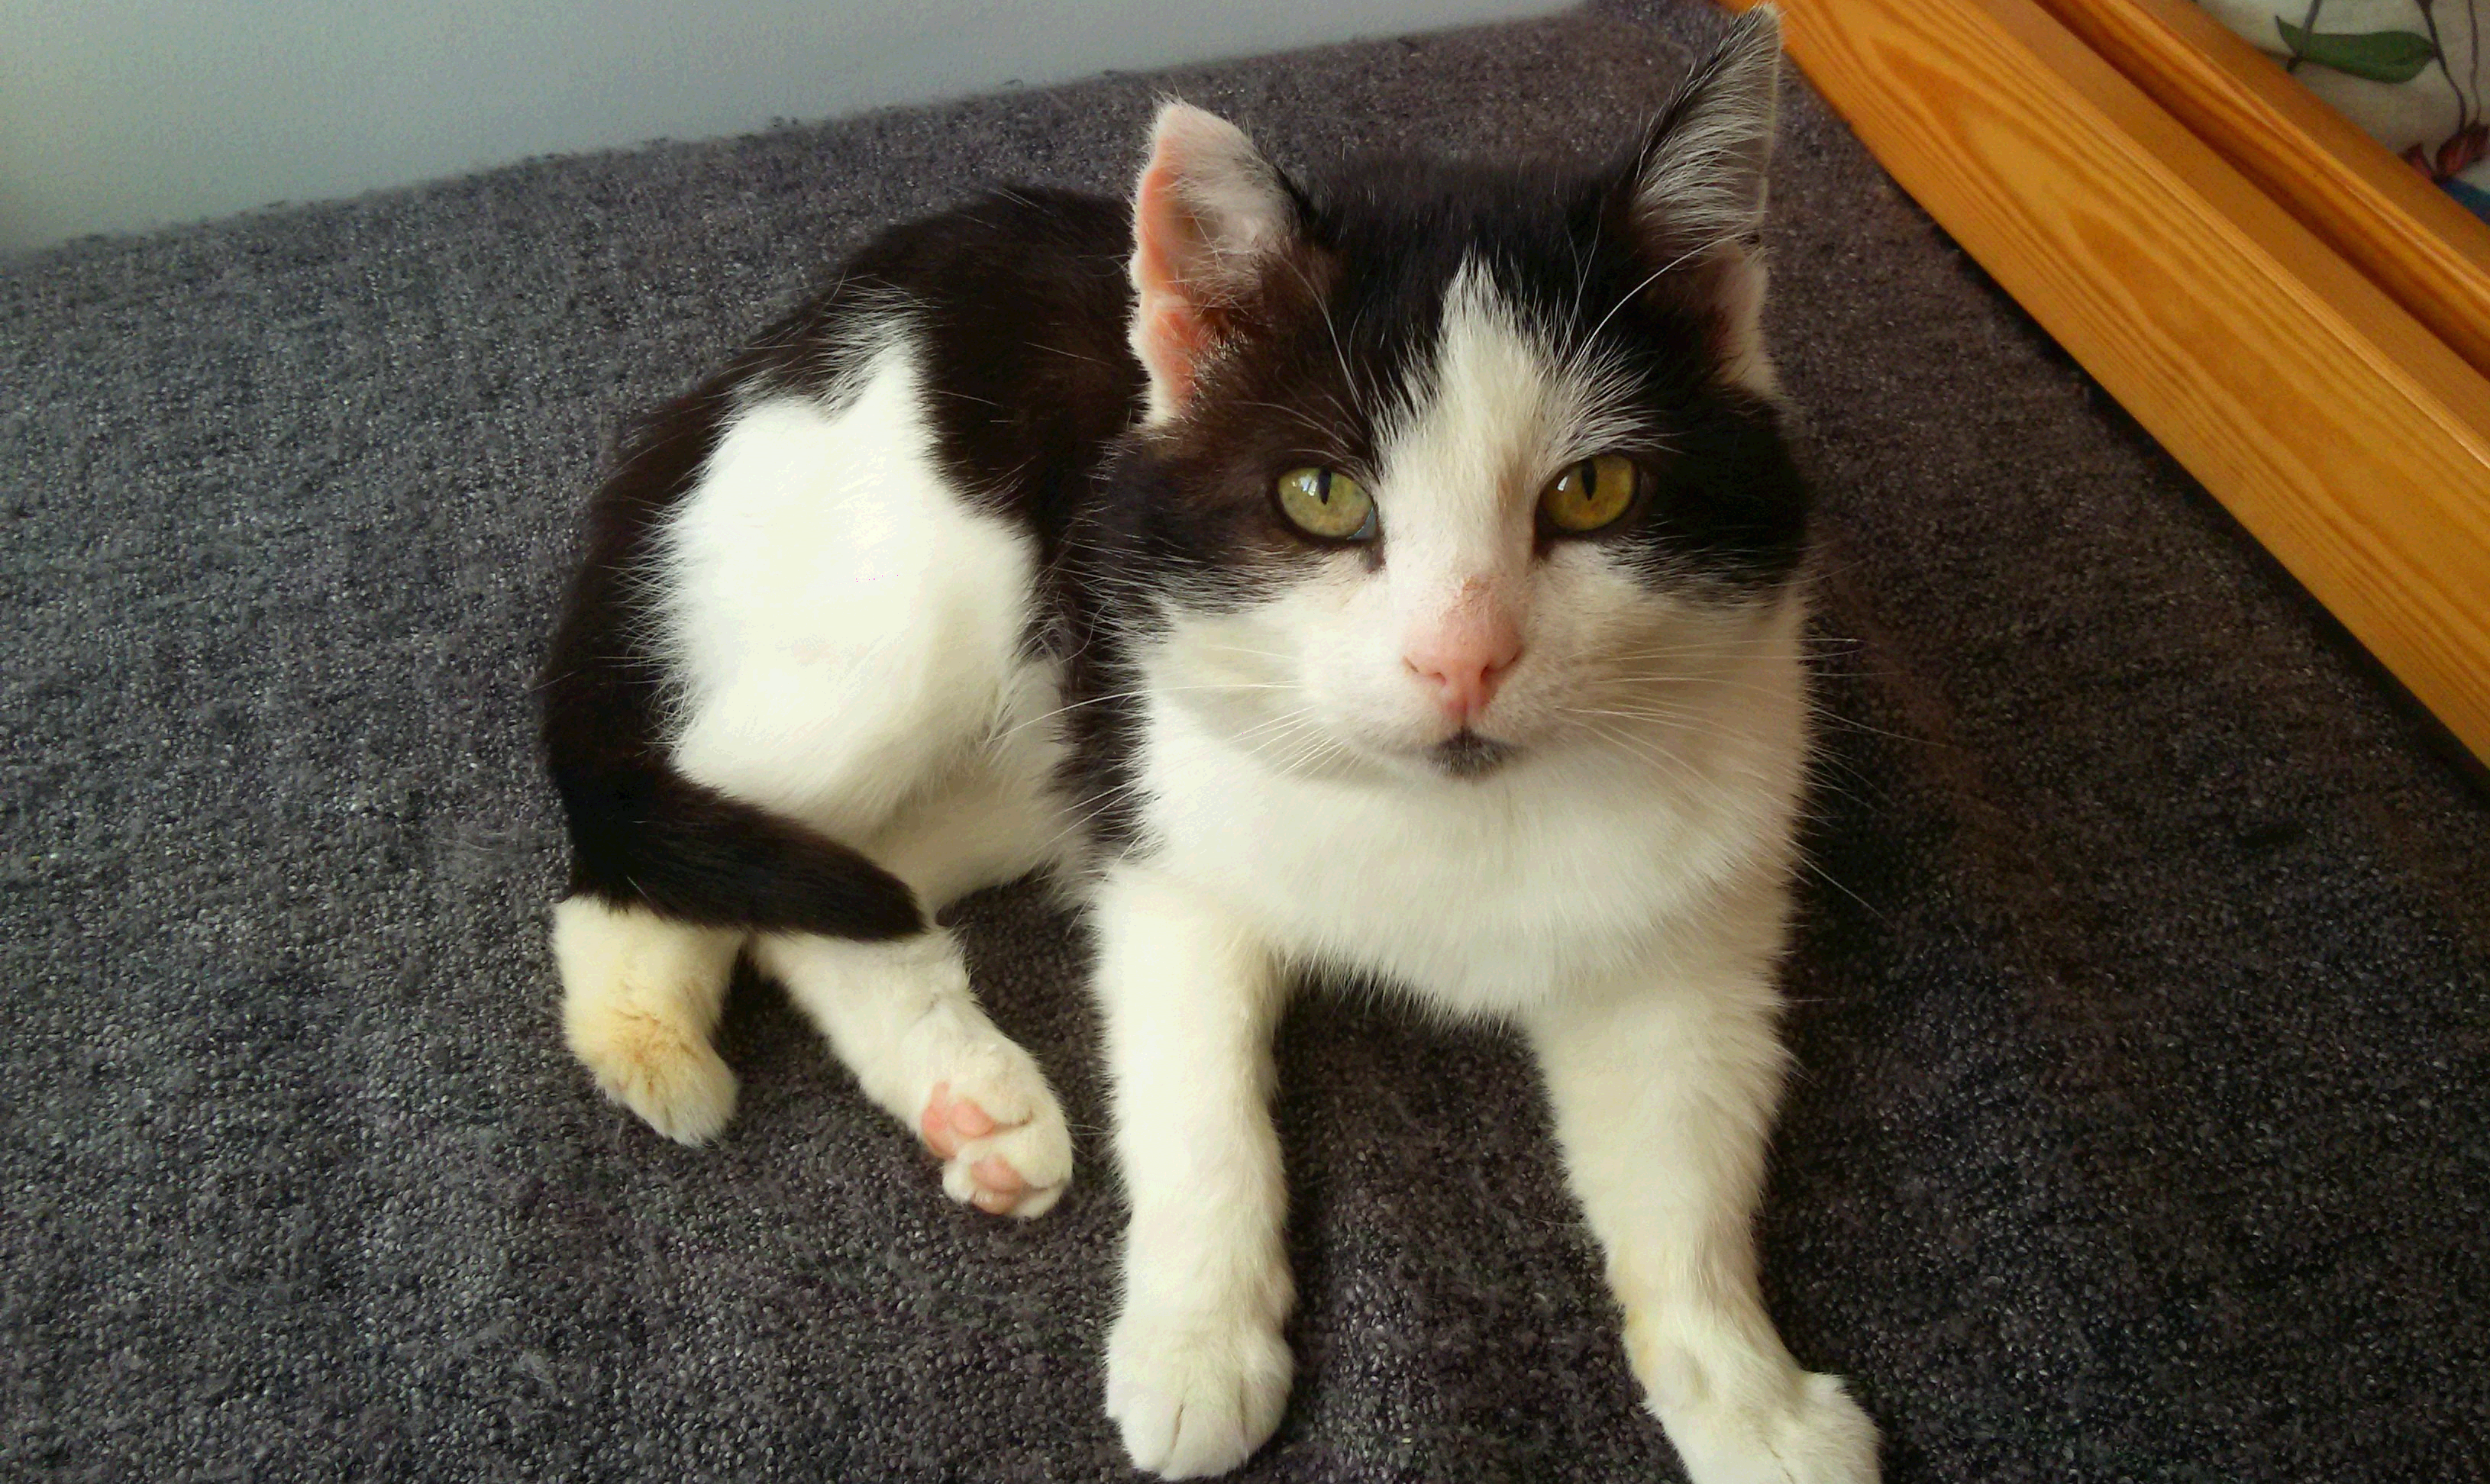
\includegraphics[width=0.7\textwidth]{pieces/kot-z-wiadomosca}
        \caption{Wynik działania algorytmu} \label{fig:stegano-rezultat}
    \end{figure}
% COLOR-ONLY END

\end{document}
